\subsection{Tipanje problema}
Obravnave se lotim z določanjem reprezentacije cevi v matrični obliki za $n$ elementov v vsaki dimenziji (zahtevam še $n \mod 3 = 0$). Za $n=27$ dobim spodnjo sliko. Poleg geometrijskih atributov sem na koncu zahteval še `črn rob' okrog cevi, kjer je hitrost ničelna.
\begin{center}
    
\includegraphics[width=0.5\textwidth]{../old/1-hiska.pdf}
\end{center}
Najprej sem poskusil Jacobijevo metodo na kvadratni cevi, da se uverim, ali je problem zastavljen pravilno.
\begin{center}
    \begin{minipage}{0.45\textwidth}
        \centering
    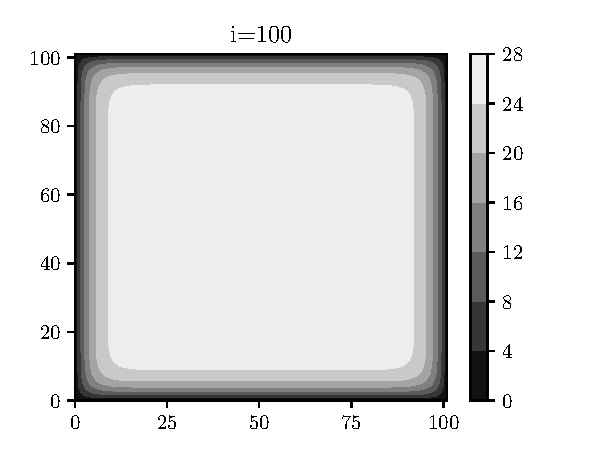
\includegraphics[width=\textwidth]{../old/../old/0-kvadratna_i100.pdf}
    {Hitrostno polje v kvadratni cevi po 100 korakih iteracije.}
    \end{minipage}\hfill
    \begin{minipage}{0.45\textwidth}
        \centering
        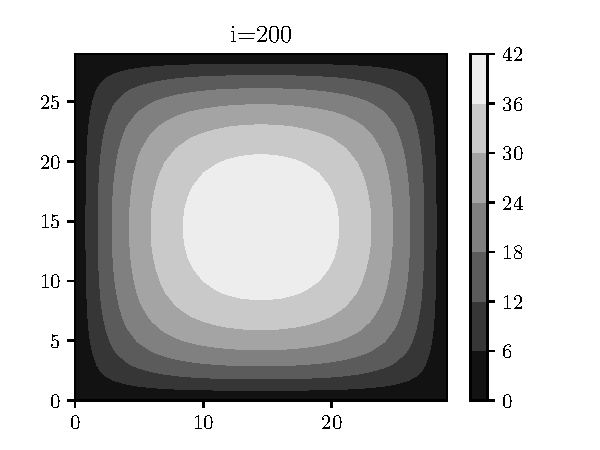
\includegraphics[width=1\textwidth]{../old/0-kvadratna_i200.pdf}
    {Hitrostno polje v kvadratni cevi po 200 korakih iteracije.}
    \end{minipage}


    \begin{minipage}{0.45\textwidth}
        \centering
    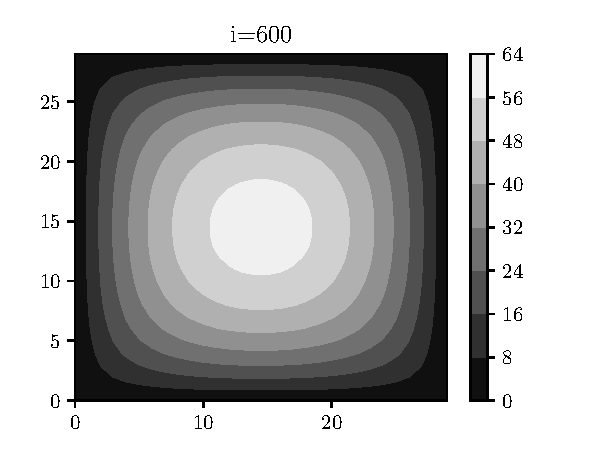
\includegraphics[width=\textwidth]{../old/0-kvadratna_i600.pdf}
    {Hitrostno polje v kvadratni cevi po 600 korakih iteracije.}
    \end{minipage}\hfill
    \begin{minipage}{0.45\textwidth}
        \centering
        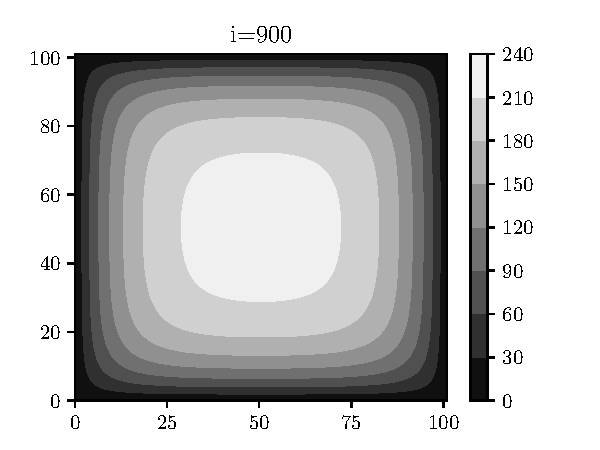
\includegraphics[width=1\textwidth]{../old/0-kvadratna_i900.pdf}
    {Hitrostno polje v kvadratni cevi po 900 korakih iteracije. }
    \end{minipage}

    \begin{minipage}{0.45\textwidth}
        \centering
    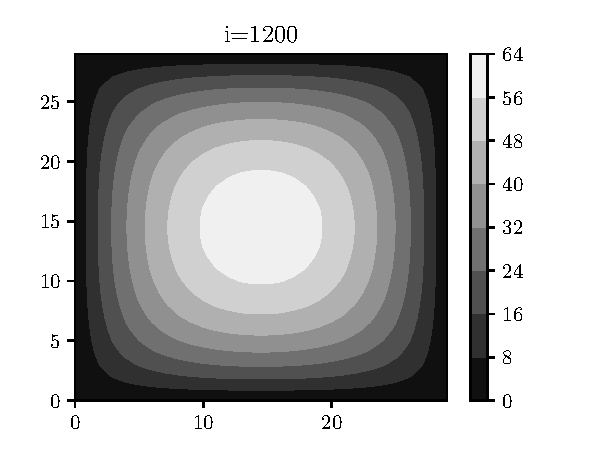
\includegraphics[width=\textwidth]{../old/0-kvadratna_i1200.pdf}
    {Hitrostno polje v kvadratni cevi po 1200 korakih iteracije.}
    \end{minipage}\hfill
    \begin{minipage}{0.45\textwidth}
        \centering
        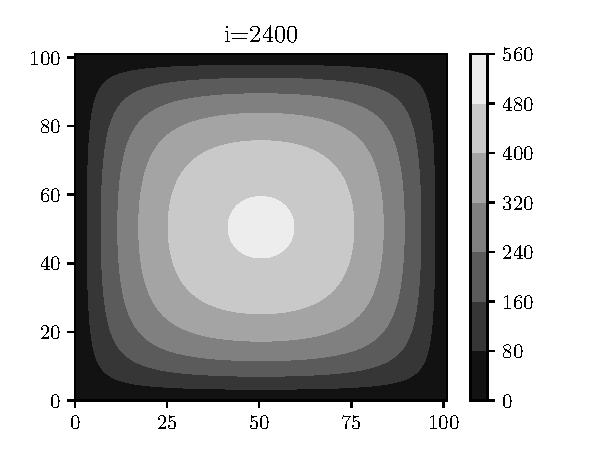
\includegraphics[width=1\textwidth]{../old/0-kvadratna_i2400.pdf}
    {Hitrostno polje v kvadratni cevi po 2400 korakih iteracije.}
    \end{minipage}
\end{center}
Validacija rezultatov je na tej točki predvsem optična, zato velja za primerjavo metod v nadaljevanju uvesti primerne metrike, denimo relativno razliko med iteracijami, ali pa kar Poiseuillov koeficient. Za začetek sem uvedel preprosto metriko, ki vrne razmerje med vsoto absolutnih razlik po elementih dveh matrik in vsoto po elementih prve matrike:
\begin{python}
def rel_err(a1: numpy.ndarray, a2: numpy.ndarray) -> float:

    return np.sum(np.abs(a1-a2).reshape(-1))/np.sum(np.abs(a1.reshape(-1)))
\end{python}
Opazim, da sprva hitro približevanje konvergenci preide v počasnejše, a monotono padanje.
\begin{center}
    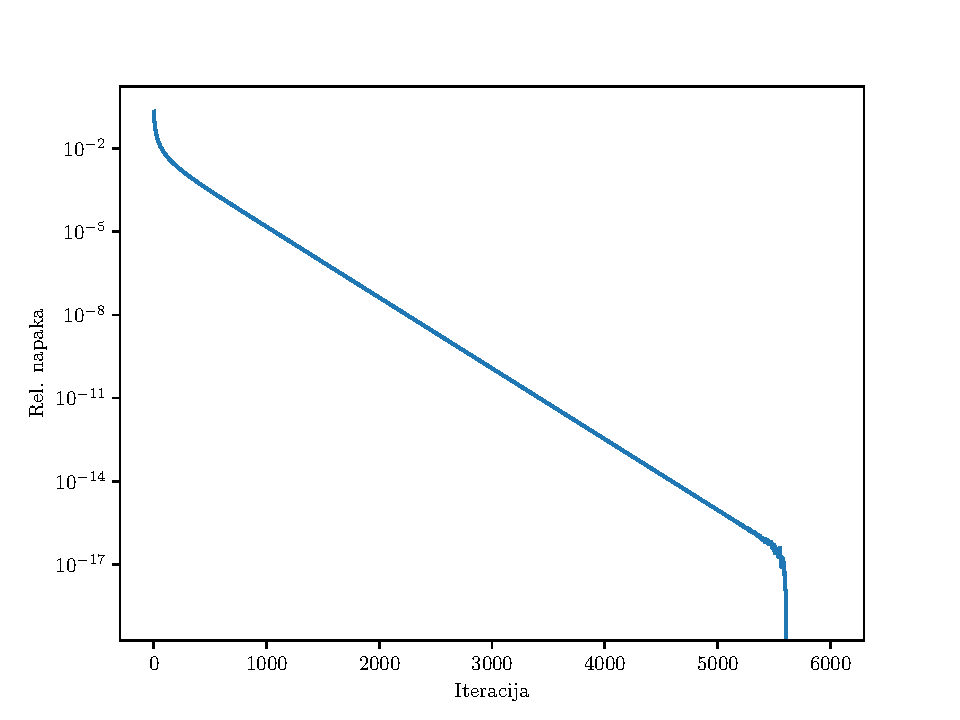
\includegraphics[width=0.5\textwidth]{../old/0-errors.pdf}
\end{center}
Nadaljujem lahko s podanim profilom cevi.
\subsection{Rešitev za podan profil cevi}
S pripravljeno matriko za profil cevi lahko postopek za kvadratno cev hitro popravim za dano cev. Nadaljnja metodologija je enaka.
\begin{center}
    \begin{minipage}{0.45\textwidth}
        \centering
    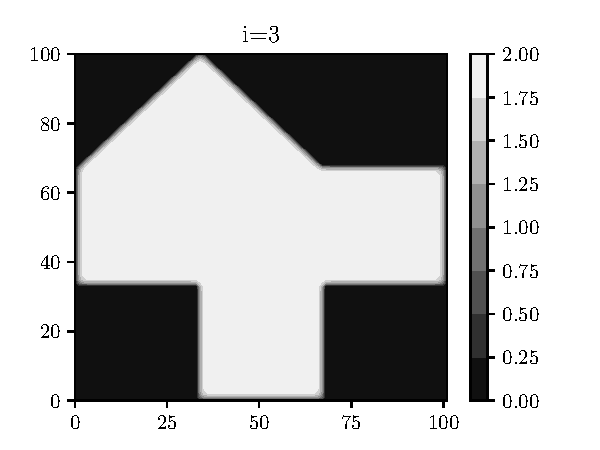
\includegraphics[width=\textwidth]{../old/1-hiska_i3.pdf}
    {Hitrostno polje v podani cevi po treh korakih iteracije.}
    \end{minipage}\hfill
    \begin{minipage}{0.45\textwidth}
        \centering
        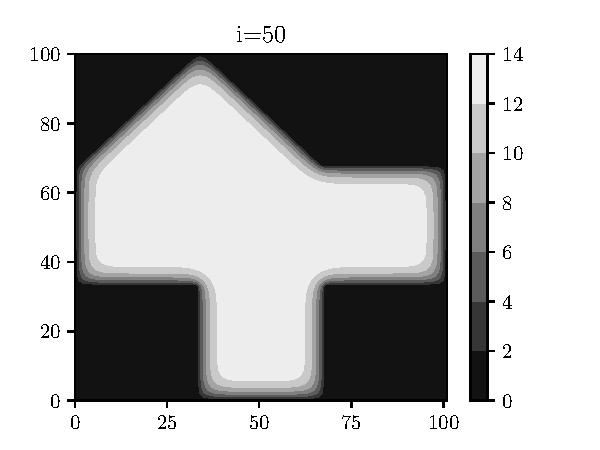
\includegraphics[width=1\textwidth]{../old/1-hiska_i50.pdf}
    {Hitrostno polje v podani cevi po 50 korakih iteracije. Opazimo enake tendence povečevanja hitrostnega polja kot pri okrogli cevi.}
    \end{minipage}

    \begin{minipage}{0.45\textwidth}
        \centering
    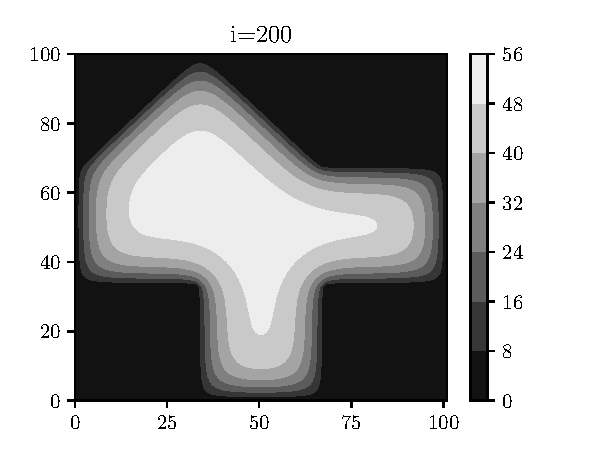
\includegraphics[width=\textwidth]{../old/1-hiska_i200.pdf}
    {Hitrostno polje v podani cevi po 200 korakih iteracije.}
    \end{minipage}\hfill
    \begin{minipage}{0.45\textwidth}
        \centering
        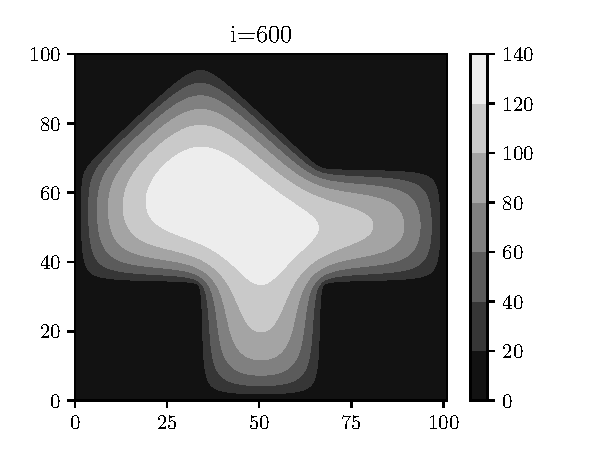
\includegraphics[width=1\textwidth]{../old/1-hiska_i600.pdf}
    {Hitrostno polje v podani cevi po 600 korakih iteracije. }
    \end{minipage}

    \begin{minipage}{0.45\textwidth}
        \centering
    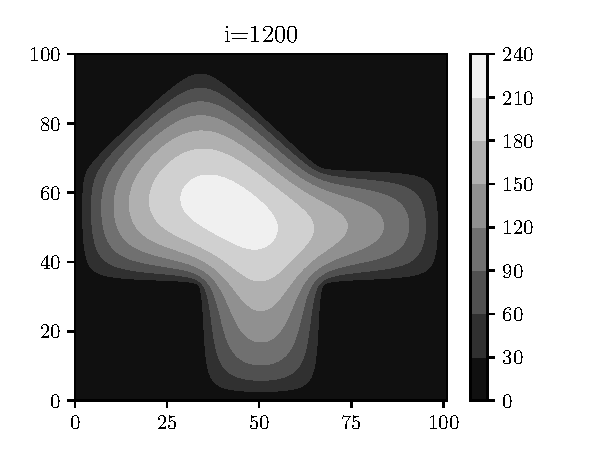
\includegraphics[width=\textwidth]{../old/1-hiska_i1200.pdf}
    {Hitrostno polje v podani cevi po 1200 korakih iteracije.}
    \end{minipage}\hfill
    \begin{minipage}{0.45\textwidth}
        \centering
        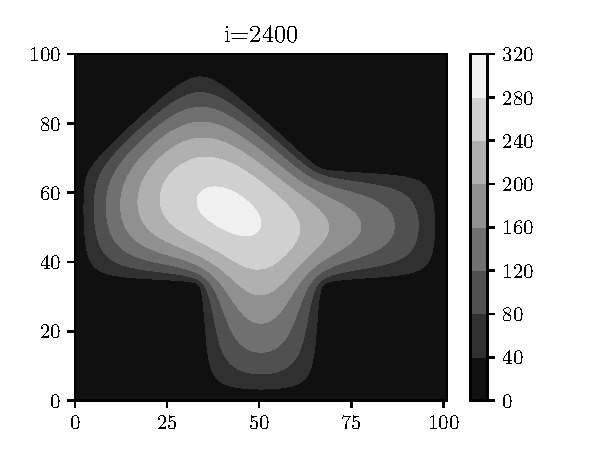
\includegraphics[width=1\textwidth]{../old/1-hiska_i2400.pdf}
    {Hitrostno polje v kvadratni cevi po 2400 korakih iteracije.}
    \end{minipage}
\end{center}
Spet lahko pogledamo hitrost konvergence. Kot je razvidno iz točke, ko razlika med zaporednima iteracijama pade na 0, je v trenutnem primeru konvergenca hitrejša.
\begin{center}
    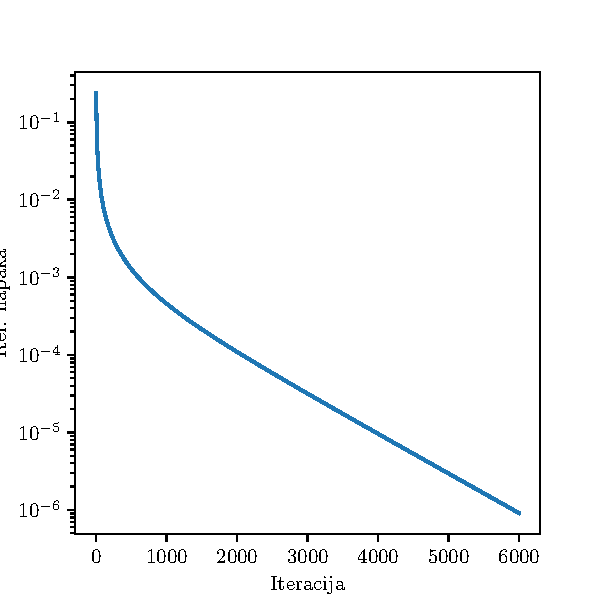
\includegraphics[width=0.5\textwidth]{../old/1-errors.pdf}
\end{center}
\subsection{Implementacija pospešene iteracijske sheme}
Nadaljeval sem z implementacijo metode~SOR. Popravljena koda je delovala odlično, evalvacija pa mi je povzročala nekaj težav. Končno sem se odločil za sledeč postopek: generiral sem `pravo' hitrostno polje s 1000 koraki iteracije, nato pa sem pri posameznih vrednostih $\omega$ z metodo SOR iteriral le 100 korakov. Rezultata sem primerjal z vsoto absolutnih razlik po elementih.
\begin{center}
    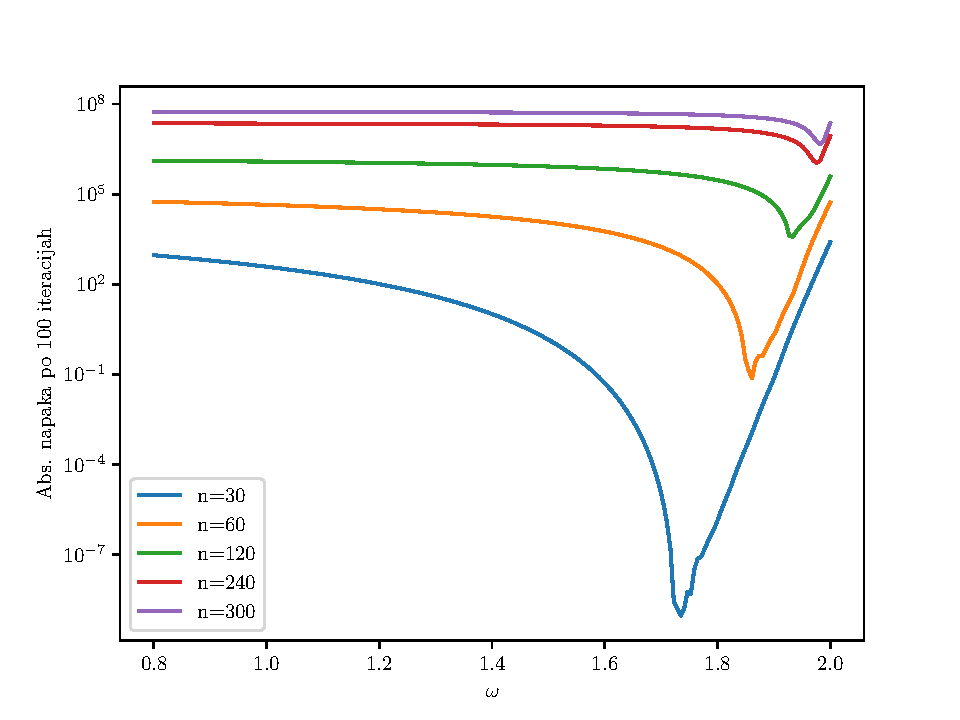
\includegraphics[width=0.7\textwidth]{../old/1-omegas.pdf}
\end{center}
Kot smo pričakovali s predavanj, je optimalna $\omega$ odvisna od dimenzije problema. Naraščanje napake (neodvisno od $\omega$) lahko pojasnimo s tem, da je matrika hitrostnega polja večja, zaradi česar je tudi razlika med `pravim' in trenutnim hitrostnim poljem večja.

Nadaljujem z uvedbo parametra $\alpha$, kot je definiran v navodilih:
\[\omega = \frac{2}{1+\alpha \frac{\pi}{N}}.\]
Kot razvidno na sliki spodaj, je zdaj optimalen pospešek invarianten od števila točk na mreži.
\begin{center}
    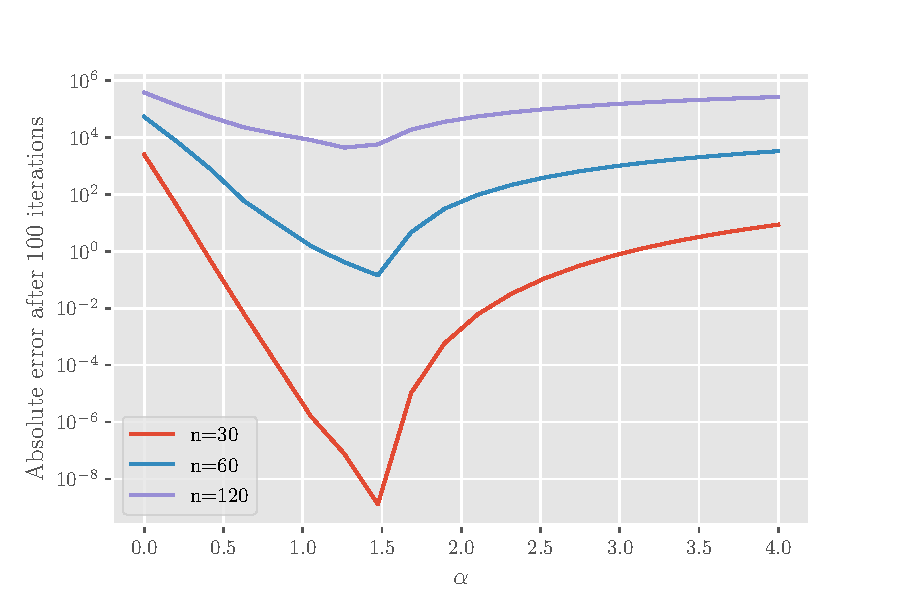
\includegraphics[width=0.7\textwidth]{../old/1-alphas.pdf}
\end{center}
\subsection{Poiseuillov koeficient}
Zdaj lahko z optimalnim pospeškom iščem Poiseuillov koeficient za dano cev. Zanj velja:

\[ \Phi_V = \iint u(x,y) \; \mathrm{d}S = \frac{C S^2}{8 \pi \eta} \dpar{p}{z}.\]

Izrazim lahko \[ C^{*} = C \eta^{-1} \dpar{p}{z},\] za presek cevi pa vzamem analitično vrednost $S = \dfrac{5}{9}.$

Za izračun $\Phi$ sem poskusil integracijo z dvodimenzionalnim Simposonom, s svojo implementacijo dvodimenzionalne verzije metode za trapezijsko integracijo \texttt{numpy.trapz}, pa tudi z rudimentarno sumacijo. Medsebojno so se vse metode razlikovale pod $0.1 \%$. Pri iteraciji sem uporabil zgoraj določen optimalen parameter $\alpha$ za pospešek iteracije.

\begin{center}
    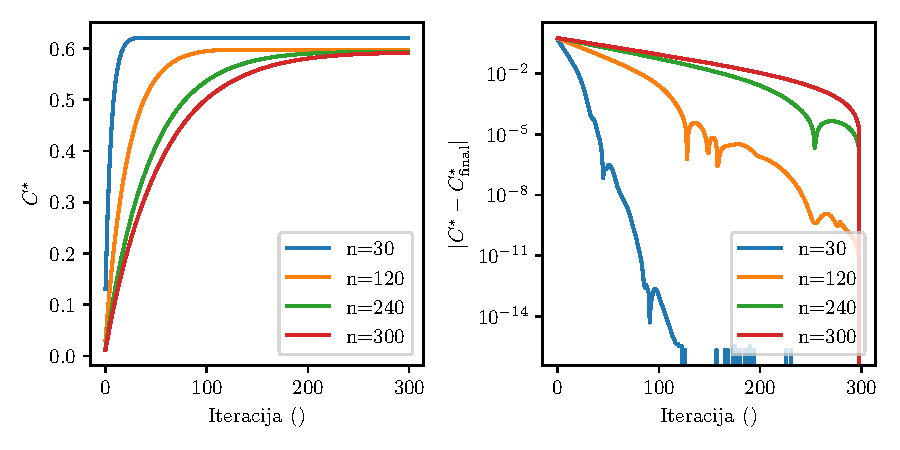
\includegraphics[width=0.9\textwidth]{../old/1-C__.pdf}


    {Vrednost modificiranega Poiseuillovega koeficienta $C^{*}$med iteriranjem in absolutne razlike med končnim in trenutnim $C^{*}$ za različna števila točk v vsaki dimenziji $n$.}
\end{center}

